%**********************************************************************%
% _                    _                       _       _
% | |__   ___ _ __ ___ | |_ ___ _ __ ___  _ __ | | __ _| |_ ___
% | '_ \ / _ \ '_ ` _ \| __/ _ \ '_ ` _ \| '_ \| |/ _` | __/ _ \
% | |_) |  __/ | | | | | ||  __/ | | | | | |_) | | (_| | ||  __/
% |_.__/ \___|_| |_| |_|\__\___|_| |_| |_| .__/|_|\__,_|\__\___|
%                                        |_|
%----------------------------------------------------------------------%
\RequirePackage{plautopatch} %日本語パッケージを使う.
\documentclass[aspectratio=169, 12pt]{beamer} %  8pt, 9pt, 10pt, 11pt, 12pt, 14pt, 17pt, 20pt
\usetheme{Copenhagen} % テーマは指定しなくともよい.
%**********************************************************************%
% フォント
%----------------------------------------------------------------------%
\usepackage{luatexja} %日本語文書の組版を行う
\usepackage[T1]{fontenc} %アクセント記号をUTF-8で使用する.
\usepackage{inconsolata-nerd-font} %等幅フォント consolas
% 和文の既定フォントをゴシックに変更
\renewcommand{\kanjifamilydefault}{\gtdefault}
% Beamerによる数式フォントの置き換えを阻止
\usefonttheme{professionalfonts} 
%**********************************************************************%
% 数
%----------------------------------------------------------------------%
\usepackage{amsmath, amssymb} % 数式パッケージ
\usepackage{mathrsfs} %筆記体 $\mathscr{H}$ $\mathscr{L}$
\usepackage{bm} % for vector
%**********************************************************************%
% 図表
%----------------------------------------------------------------------%
\usepackage{here} %[H]オプション : 図表を文中のその場所に配置
\usepackage{ulem} % for \sout{} 取り消し線
\usepackage{booktabs} % \toprule \midrule \bottomrule
\usepackage{xcolor} %色
\usepackage{comment} %\begin{comment} \end{comment}でコメントアウト
\usepackage{boites} %ボックス内で改ページ可 
\usepackage{here, amsmath, latexsym, amssymb, bm, ascmac, mathtools, multicol, tcolorbox, subfig}

%**********************************************************************%
%      _                                       _
%   __| | ___   ___ _   _ _ __ ___   ___ _ __ | |_
%  / _` |/ _ \ / __| | | | '_ ` _ \ / _ \ '_ \| __|
% | (_| | (_) | (__| |_| | | | | | |  __/ | | | |_
%  \__,_|\___/ \___|\__,_|_| |_| |_|\___|_| |_|\__|
%**********************************************************************%



\begin{document}
%---------------------------------------------------------------
% タイトルスライド
%! 聞き流し数学1
\title{聞き流し数学I}
\author[物理の計算屋]{物理の計算屋}
\date{}
\frame{\maketitle} % タイトルページ
%---------------------------------------------------------------
% スライド2枚目以降
\begin{frame}{整数の加法・減法・乗法}
    %!  整数の加法・減法・乗法, 加法の交換法則AプラスBイコールBプラスA, 乗法の交換法則ABイコールBA, 加法の結合法則括弧AプラスBプラスCイコールC括弧プラスBプラスA, 乗法の結合法則括弧ABCイコールA括弧BC, 分配法則A括弧BプラスCイコールABプラスAC, 括弧AプラスBCイコールACプラスBC
    \begin{table}[h]
        \centering
        \begin{tabular}{ccc}
                 & 加法                                                 & 乗法              \\
            交換法則 & $ A+B=B+A $                                        & $ AB=BA $       \\
            結合法則 & $ (A+B)+C=C+(B+A) $                                & $ (AB)C=A(BC) $ \\
                 &                                                    &                 \\
            \\
            \\
            分配法則 & \multicolumn{2}{c}{$A(B+C)=AB+AC$, $(A+B)C=AC+BC$}                   \\
        \end{tabular}
    \end{table}
\end{frame}

%---------------------------------------------------------------
\begin{frame}{指数法則}
    %! 指数法則, aのm乗aのn乗イコールaのmプラスn乗, aのm乗のn乗イコールaのmn乗, abのn乗イコールaのn乗bのn乗
    \begin{eqnarray*}
        a^ma^n&=&a^{m+n} \\
        (a^m)^n&=&a^{mn} \\
        (ab)^n&=&a^nb^n
    \end{eqnarray*}
\end{frame}

%---------------------------------------------------------------
\begin{frame}{展開の公式, 因数分解}
    %! 展開の公式, 因数分解, 括弧aプラスb2乗イコールa2乗プラス2abプラスb2乗, 括弧aマイナスb2乗イコールa2乗マイナス2abプラスb2乗, 括弧aプラスb括弧aマイナスbイコールa2乗プラスb2乗, 括弧xプラスa括弧xプラスbイコールx2乗プラス括弧aプラスbxプラスb2乗, 括弧axpぅラスb括弧cxプラスdイコールacx2乗プラス括弧adプラスbcxプラスbd, 括弧aプラスb括弧a2乗マイナスabプラスb2乗イコールa3乗プラスb3乗, 括弧aマイナスb括弧a2乗プラスabプラスb2乗イコールa3乗マイナスb3乗, 括弧aプラスb3乗イコールa3乗プラス3a2乗bプラス3ab2乗プラスb3乗, 括弧aマイナスb3乗イコールa3乗マイナス3a2乗bプラス3ab2乗マイナスb3乗
    \begin{eqnarray*}
        (a+b)^2&=&a^2+2ab+b^2 \\
        (a-b)^2&=&a^2-2ab+b^2 \\
        (a+b)(a-b)&=&a^2+b^2 \\
        (x+a)(x+b)&=&x^2+(a+b)x+b^2 \\
        (ax+b)(cx+d)&=&acx^2+(ad+bc)x+bd \\
        (a+b)(a^2-ab+b^2)&=&a^3+b^3 \\
        (a-b)(a^2+ab+b^2)&=&a^3-b^3 \\
        (a+b)^3&=&a^3+3a^2b+3ab^2+b^3 \\
        (a-b)^3&=&a^3-3a^2b+3ab^2-b^3
    \end{eqnarray*}
\end{frame}
%---------------------------------------------------------------
\begin{frame}{実数の構造}
    %! 実数の構造, 実数は有理数と無理数に分かれます. 有理数は整数と有限小数, 循環小数に分かれます. 整数は自然数, ゼロ, 負の整数に分かれます. 有限小数と無限小数は分数で表せます. 
    \begin{figure}[htbp]
        \begin{center}
            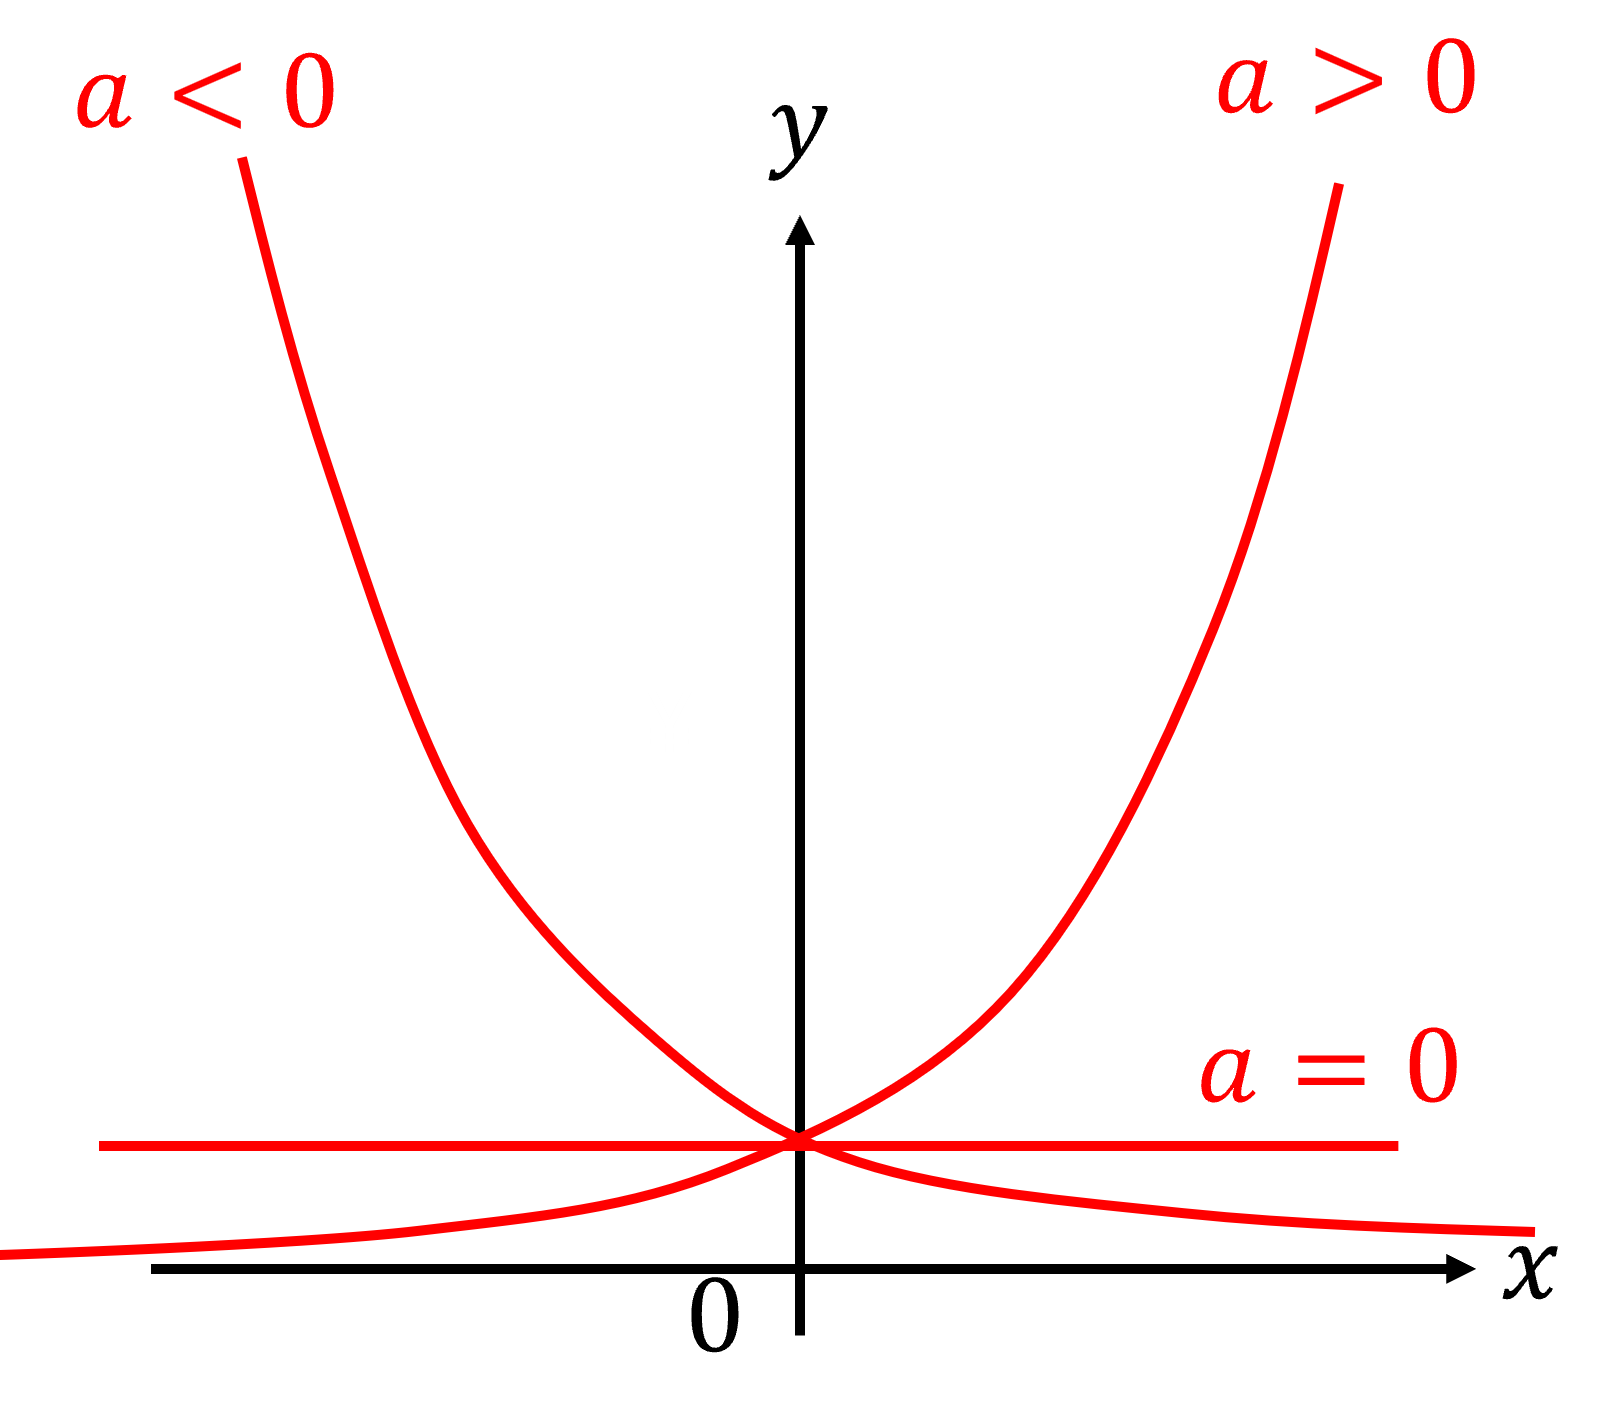
\includegraphics[width=100mm]{fig/1.png}
        \end{center}
    \end{figure}
\end{frame}

%---------------------------------------------------------------
\begin{frame}{絶対値の性質}
    %! 絶対値の性質, aダイナリイコールゼロのとき, 絶対値aイコールa, aショウナリイコールゼロのとき, 絶対値aイコールマイナスa
    \begin{center}
        $ a \geq 0 $ のとき $|a|=a$ \par
        $ a \leq 0 $ のとき $|a|=-a$ \par
    \end{center}
\end{frame}
%---------------------------------------------------------------
\begin{frame}{平方根の性質}
    %! 平方根の性質, aダイナリイコールゼロのとき, ルートa2乗イコールa, 括弧マイナスルートa2乗イコールa, ルートaダイナリイコールゼロ, ルートa2乗イコールa, aショウナリイコールゼロのとき, ルートa2乗イコールマイナスa, aダイナリゼロ, bダイナリゼロ, kダイナリゼロのとき, ルートaルートbイコールルートab, ルートb分のルートaイコールルートb分のa, k2乗aイコールkルートa
    $ a \geq 0 $ のとき \par
    \begin{center}
        $(\sqrt{a})^2=a$, $(-\sqrt{a})^2=a$, $\sqrt{a}\geq 0, \sqrt{a^2}=a$
    \end{center}
    $ a \leq 0 $ のとき \par
    \begin{center}
        $\sqrt{a^2}=-a$
    \end{center}
    $ a > 0$, $b>0$, $k>0$ のとき \par
    \begin{eqnarray*}
        \sqrt{a}\sqrt{b}&=&\sqrt{ab} \\
        \frac{\sqrt{a}}{\sqrt{b}}&=&\sqrt{\frac{a}{b}} \\
        \sqrt{k^2a}&=&k\sqrt{a}
    \end{eqnarray*}
\end{frame}
%---------------------------------------------------------------
\begin{frame}{2重根号のはずし方}
    %! 2重根号のはずし方, 文字はすべて正の整数とする. ルートpプラスkルートqはルート括弧aプラスbプラスマイナスルート2abに変形し, ルート括弧aプラスbプラスルート2abイコールルートaプラスb, ルート括弧aプラスbプラスマイナスルート2abイコールルートaマイナスb
    文字はすべて正の整数とする \par
    $\sqrt{p+k\sqrt{q}}$ は$\sqrt{(a+b)\pm 2\sqrt{ab}}$に変形し, \par
    \begin{eqnarray*}
        \sqrt{(a+b)+2\sqrt{ab}}&=&\sqrt{a}+\sqrt{b} \\
        \sqrt{(a+b)-2\sqrt{ab}}&=&\sqrt{a}-\sqrt{b}
    \end{eqnarray*}
\end{frame}
%---------------------------------------------------------------
\begin{frame}{不等式の性質}
    %! 不等式の性質, aショウナリbならば, aプラスcショウナリbプラスc, aマイナスcショウナリbマイナスc, aショウナリb, cダイナリゼロならばacショウナリbc, c分のaショウナリc分のb, aショウナリb, cショウナリゼロならばacダイナリbc, c分のaダイナリc分のb, aショウナリb, bショウナリcならばaショウナリc
    \begin{eqnarray*}
        a<b&ならば&a+c<b+c, a-c<b-c \\
        a<b, c>0&ならば&ac<bc, \frac{a}{c}<\frac{b}{c} \\
        a<b, c<0&ならば&ac>bc, \frac{a}{c}>\frac{b}{c} \\
        a<b, b<c&ならば&a<c
    \end{eqnarray*}
\end{frame}
%---------------------------------------------------------------
\begin{frame}{絶対値を含む方程式, 不等式}
    %! 絶対値を含む方程式, 不等式, 絶対値AイコールAただし Aがゼロ以下のとき, マイナスAただしAがゼロ未満のとき. 簡便法 cダイナリゼロのとき方程式, 絶対値xイコールcの解はxイコールプラスマイナスc, 絶対値xショウナリcの解はマイナスcショウナリxショウナリc, 絶対値xダイナリcの解はxショウナリマイナスc, cショウナリx
    場合分け\par
    \begin{eqnarray*}
        |A|=
        \begin{cases}
            A (A\geq 0) \\
            -A (A < 0)
        \end{cases}
    \end{eqnarray*}
    簡便法 $c>0$のとき方程式 \par
    \begin{eqnarray*}
        |x|=c&の解は&x=\pm c \\
        |x|<c&の解は&-c<x<c \\
        |x|>c&の解は&x<-c, c<x
    \end{eqnarray*}
\end{frame}
%---------------------------------------------------------------
\begin{frame}{集合の基本}
    %! 集合の基本, Uは全体集合でABCはUの部分集合とする. 部分集合とはAがBに含まれる, つまり要素xがAに含まれるならばxがBに含まれるが成り立ちます. 相当とはAイコールB, つまりAがBに含まれて, かつ, BがAに含まれる状態をいいます. 共通部分はAキャップBイコールx, xがAに含まれて, かつ, xがBに含まれます. 和集合AカップBイコールx, xがAに含まれるか, または, xがBに含まれます. 補集合aバーイコールx, xがUに含まれて, かつxはAに含まれません.
    $U$は全体集合で$A$, $B$, $C$は$U$の部分集合とする \par
    部分集合 $A\subset B$ \par
    \begin{center}
        「$x \in A$ならば$x\in B$」が成り立つ\par
    \end{center}
    相当 $A=B$ \par
    \begin{center}
        「$A\subset B$かつ$B\subset A$」が成り立つ \par
    \end{center}

    共通部分 $A\cap B = \{x|x\in A かつ x \in B\}$ \par
    和集合\space\space\space\space $A\cup B = \{x|x\in A または x \in B \}$ \par
    補集合\space\space\space\space\space\space\space\space\space\space $\bar{A}=\{x|x\in U かつ x\notin A\}$
\end{frame}
%---------------------------------------------------------------
\begin{frame}{ド・モルガンの法則}
    %! ド・モルガンの法則, AカップBバーイコールAバーキャップBバー, AキャップBバーイコールAバーカップBバー, AカップBカップCバーイコールAバーキャップBバーキャップCバー, AキャップBキャップCイコールAバーカップBバーカップCバー
    \begin{eqnarray*}
        \overline{A\cup B}&=&\bar{A}\cap \bar{B} \\
        \overline{A\cap B}&=&\bar{A}\cup \bar{B} \\
        \overline{A\cup B\cup C}&=&\bar{A}\cap\bar{B}\cap\bar{C} \\
        \overline{A\cap B\cap C}&&\bar{A}\cup\bar{B}\cup\bar{C}
    \end{eqnarray*}
\end{frame}
%---------------------------------------------------------------
\begin{frame}{命題と条件}
    %! 命題と条件, 真の場場合証明する. ぎの場合反例を挙げる.
    \begin{center}
        真の場合: 証明する \par
        偽の場合: 反例を1つあげる
    \end{center}
\end{frame}
%---------------------------------------------------------------
\begin{frame}{必要・十分条件}
    %! 必要・十分条件, ふたつの条件p, qについてp矢印qが真であるとき, qはpであるための必要条件, pはqであるための十分条件, p矢印q, q矢印pが共に真であるとき, qはpであるための必要十分条件.
    2つの条件$p$, $q$について \par
    $p \Rightarrow q$が真であるとき \par
    \begin{center}
        $q$は$p$\space であるための必要条件 \par
        $p$は$q$\space であるための十分条件
    \end{center}
    $p \Rightarrow q$, $q \Rightarrow p$が共に真であるとき \par
    \begin{center}
        $q$は$p$ ($p$は$q$)であるための必要十分条件
    \end{center}
\end{frame}
%---------------------------------------------------------------
\begin{frame}{命題の逆, 対偶, 裏}
    %! 命題の逆, 対偶, 裏, 命題とその対偶の真偽は一致する.
    \begin{figure}[htbp]
        \begin{center}
            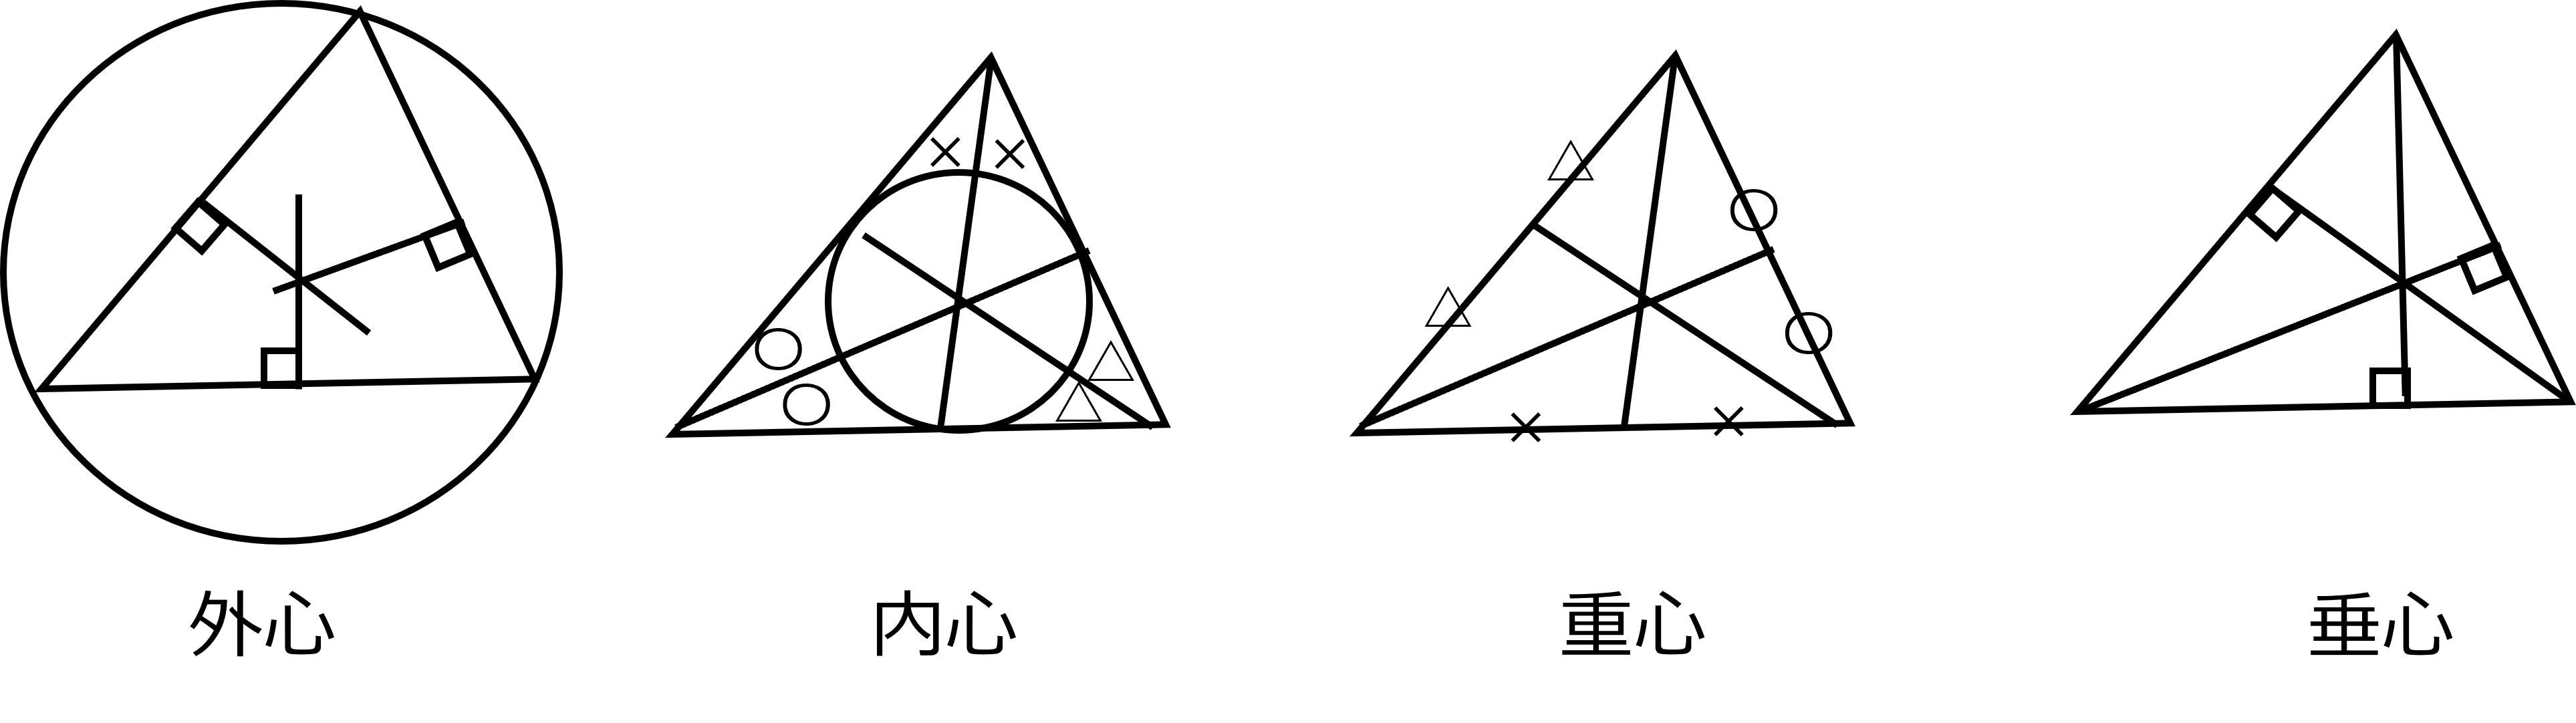
\includegraphics[width=100mm]{fig/2.png}
        \end{center}
    \end{figure}
    \begin{center}
        命題とその対偶の真偽は一致する
    \end{center}
\end{frame}

%---------------------------------------------------------------
\begin{frame}{$y=a(x-p)^2+q$ $ (a\neq 0)$ のグラフ}
    %! yイコールa括弧xマイナスp2乗プラスqのグラフ, 頂点pq, 軸が直線xイコールpの放物線, aダイナリゼロなら下にとつ, aショウナリゼロなら上にとつ
    \begin{center}
        頂点 ($p$, $q$), 軸が直線 $x=p$ の放物線 \par
        $a>0$なら下に凸, $a<0$なら上に凸
    \end{center}
\end{frame}

%---------------------------------------------------------------
\begin{frame}{$y=ax^2+bx+c$ $ (a\neq 0)$のグラフ}
    %! yイコールax2乗プラスbxプラスcのグラフ, 右辺を平方完成してyイコールa括弧xプラス2a分のb2乗マイナス4a分のb2乗マイナス4ac, 頂点マイナス2a分のb, マイナス4a分のbマイナス4ac, 軸が直線xイコールマイナス2a分のbの放物線
    右辺を平方完成して \par
    \begin{eqnarray*}
        y=a\left( x+\frac{b}{2a} \right) ^2 -\frac{b^2-4ac}{4a}
    \end{eqnarray*}
    \begin{center}
        頂点$\left(-\frac{b}{2a}, -\frac{b-4ac}{4a}\right)$,
        軸が直線 $x=-\frac{b}{2a}$の放物線
    \end{center}
\end{frame}
%---------------------------------------------------------------
\begin{frame}{平行移動}
    %! 平行移動, x方向にp, y方向にqの平行移動で点abはaプラスp, bプラスq, グラフyイコールfxはyマイナスqイコールfxマイナスp
    \begin{eqnarray*}
        x方向にp, y方向にqの平行移動で \\
        点(a,b)&\rightarrow& (a+p, b+q), \\
        グラフ y=f(x) &\rightarrow& y-q=f(x-p)
    \end{eqnarray*}
\end{frame}
%---------------------------------------------------------------
\begin{frame}{対称移動}
    %! 対称移動, x軸に対して対称移動, aマイナスb, yイコールマイナスfx, y軸に対して対称移動マイナスab, yイコールfマイナスx, 原点に対して対称移動マイナスaマイナスb, yイコールマイナスfマイナスx
    \begin{table}[h]
        \centering
        \begin{tabular}{cccc}
                     & $x$軸      & $y$軸      & 原点         \\
            $(a,b)$  & $(a, -b)$ & $(-a, b)$ & $(-a, -b)$ \\
            $y=f(x)$ & $y=-f(x)$ & $y=f(-x)$ & $y=-f(-x)$
        \end{tabular}
    \end{table}
\end{frame}
%---------------------------------------------------------------
\begin{frame}{2次関数$y=ax^2+bx+c$の最大・最小}
    %! 2次関数ax2乗プラスbxプラスcの最大・最小平方完成してyイコールa括弧xマイナスp2乗プラスqの形にする. aダイナリゼロのとき, xイコールpで最小値q, 最大値はない. aショウナリゼロのとき, xイコールpで最大値q, 最小値はない.
    \begin{center}
        平方完成して$y=a(x-p)^2+q$の形にする \par
        $a>0$のとき, $x=p$で最小値$q$, 最大値はない\par
        $a<0$のとき,  $x=p$で最大値$q$, 最小値はない
    \end{center}
\end{frame}
%---------------------------------------------------------------
\begin{frame}{2次関数$y=ax^2+bx+c$ $(h\leq x \leq k)$の最大・最小}
    %!2次関数ax2乗プラスbxプラスcの最大・最小hショウナリxショウナリkの場合, aダイナリゼロ, 下にとつの場合, 区間の内に頂点があるとき, 頂点で最小, 頂点から遠い区間の端で最大, 区間の内に頂点がないとき, 頂点に近い区間の端で最小, 遠い端で最大.
    $a>0$ (下に凸)の場合, \par
    1. 区間の内に頂点があるとき,  頂点で最小, 頂点から遠い区間の端で最大 \par
    2. 区間の内に頂点がないとき,  頂点に近い区間の端で最小, 遠い端で最大
\end{frame}
%---------------------------------------------------------------
\begin{frame}{2次関数の決定}
    %! 2次関数の決定, 与えられた条件が放物線や頂点の軸, yイコールa括弧xマイナスp2乗プラスqとおく, グラフが通3点, yイコールax2乗プラスbxプラスcとおく
    与えられた条件が\par
    1. 放物線の頂点や軸 \par
    \begin{center}
        → $y=a(x-p)^2+q$とおく \par
    \end{center}
    2. グラフが通る3点 \par
    \begin{center}
        → $y=ax^2+bx+c$とおく
    \end{center}
\end{frame}

%---------------------------------------------------------------
\begin{frame}{2次方程式の実数解の個数}
    %! 2次方程式の実数解の個数, 2次方程式ax2乗プラスbxプラスcイコールゼロの判別式Dイコールb2乗マイナス4acに対しこの方程式が異なる2つの実数解を持つ, 同値, Dダイナリゼロ, ただ一つの実数解, じゅう解をもつ, 同値, Dイコールゼロ, 実数解をもたない, 同値, Dショウナリゼロ
    2次方程式$ax^2+bx+c=0$の判別式$D=b^2-4ac$に対し, \par
    この方程式が \par
    \begin{eqnarray*}
        異なる2つの実数解をもつ &\Leftrightarrow& D>0 \\
        ただ1つの実数解 (重解) をもつ &\Leftrightarrow& D=0 \\
        実数解をもたない &\Leftrightarrow& D<0
    \end{eqnarray*}
\end{frame}
%---------------------------------------------------------------
\begin{frame}{2次関数$y=ax^2+bx+c$のグラフと$x$軸}
    %! 2次関数ax2乗プラスbxプラスcのグラフとx軸, 2次関数yイコールax2乗プラスbxプラスcのグラフをCとする. 判別式Dイコールb2乗マイナス4acとすると, Dダイナリゼロ, 同値, Cはx軸と異なる2点で交わる. Dイコールゼロ, 同値, Cはx軸と1点で接する. Dショウナリゼロ, 同値, Cはx軸と共有点を持たない.
    2次関数$y=ax^2+bx+c$のグラフを$C$とする. 判別式$D=b^2-4ac$とすると \par
    \begin{eqnarray*}
        D>0&\Leftrightarrow& Cはx軸と異なる2点で交わる \\
        D=0&\Leftrightarrow& Cはx軸と1点で接する \\
        D<0&\Leftrightarrow& Cはx軸と共有点をもたない
    \end{eqnarray*}
\end{frame}
%---------------------------------------------------------------
\begin{frame}{$ax^2+bx+c>0$, $ax^2+bx+c<0$の解}
    %! ax2乗プラスbxプラスcダイナリゼロ, ax2乗プラスbxプラスcショウナリゼロの解, 2次方程式ax2乗プラスbxプラスcイコールゼロがことなる実数解アルファ, ベータを持ち, アルファショウナリベータとする. aダイナリゼロの場合, ax2乗プラスbxプラスcダイナリゼロの解はxショウナリアルファ, ベータショウナリx, ax2乗プラスbxプラスcショウナリゼロの解はアルファショウナリxショウナリベータ
    2次方程式$ax^2+bx+c=0$が異なる2つの実数解$\alpha$, $\beta$を持ち, $\alpha<\beta$とする \par
    $a>0$の場合, \par
    \begin{eqnarray*}
        ax^2+bx+c>0&の解は&x<\alpha, \beta<x \\
        ax^2+bx+c<0&の解は&\alpha<x<\beta
    \end{eqnarray*}
\end{frame}
%---------------------------------------------------------------
\begin{frame}{$(x-a)^2>0$, $(x-a)^2<0$の解}
    %! 括弧xマイナスa2乗ダイナリゼロ, 括弧xマイナスa2乗ショウナリゼロの解, xマイナスa2乗ショウナリゼロの解はない. xマイナスa2乗ショウナリイコールゼロの解はxイコールa, xマイナスa2乗ダイナリゼロの解はa以外のすべての実数, xマイナスa2乗ダイナリイコールゼロの解はすべての実数
    \begin{eqnarray*}
        (x-a)^2<0&の解は&ない\\
        (x-a)^2\leq 0&の解は&x=a \\
        (x-a)^2>0&の解は&a 以外のすべての実数 \\
        (x-a)^2\geq 0&の解は&すべての実数
    \end{eqnarray*}
\end{frame}
%---------------------------------------------------------------
\begin{frame}{放物線と$x$軸の共有点の位置}
    %! 放物線とx軸の共有点の位置, fxイコールax2乗プラスbxプラスc, ただしaノットイコールゼロ, Dイコールb2乗マイナス4acとする放物線yイコールfxがx軸とxイコールアルファ, ベータ, ただし, アルファ, ショウナリ,ベータで共有点を持つとする. aダイナリゼロのとき, アルファダイナリk, ベータショウナリk, 同値, Dダイナリイコールゼロ, 軸ダイナリk, fkダイナリゼロ, アルファショウナリk, ベータショウナリk 同値, Dダイナリイコールゼロ, 軸ショウナリk, fkダイナリゼロ, アルファショウナリkショウナリ, ベータ, 同値,fkショウナリゼロ
    $f(x)=ax^2+bx+c$ $(a\neq 0)$, $D=b^2-4ac$とする.
    放物線 $y=f(x)$が$x$軸と$x=\alpha, \beta$ $(\alpha\leq \beta)$で共有点を持つとする
    $a>0$のとき,
    \begin{eqnarray*}
        \alpha>k, \beta<k &\Leftrightarrow& D\geq 0, 軸\space >k, f(k)>0 \\
        \alpha<k, \beta<k &\Leftrightarrow& D\geq 0, 軸\space <k, f(k)>0 \\
        \alpha<k<\beta &\Leftrightarrow& f(k)<0 \\
    \end{eqnarray*}
    \begin{figure}[htbp]
        \begin{center}
            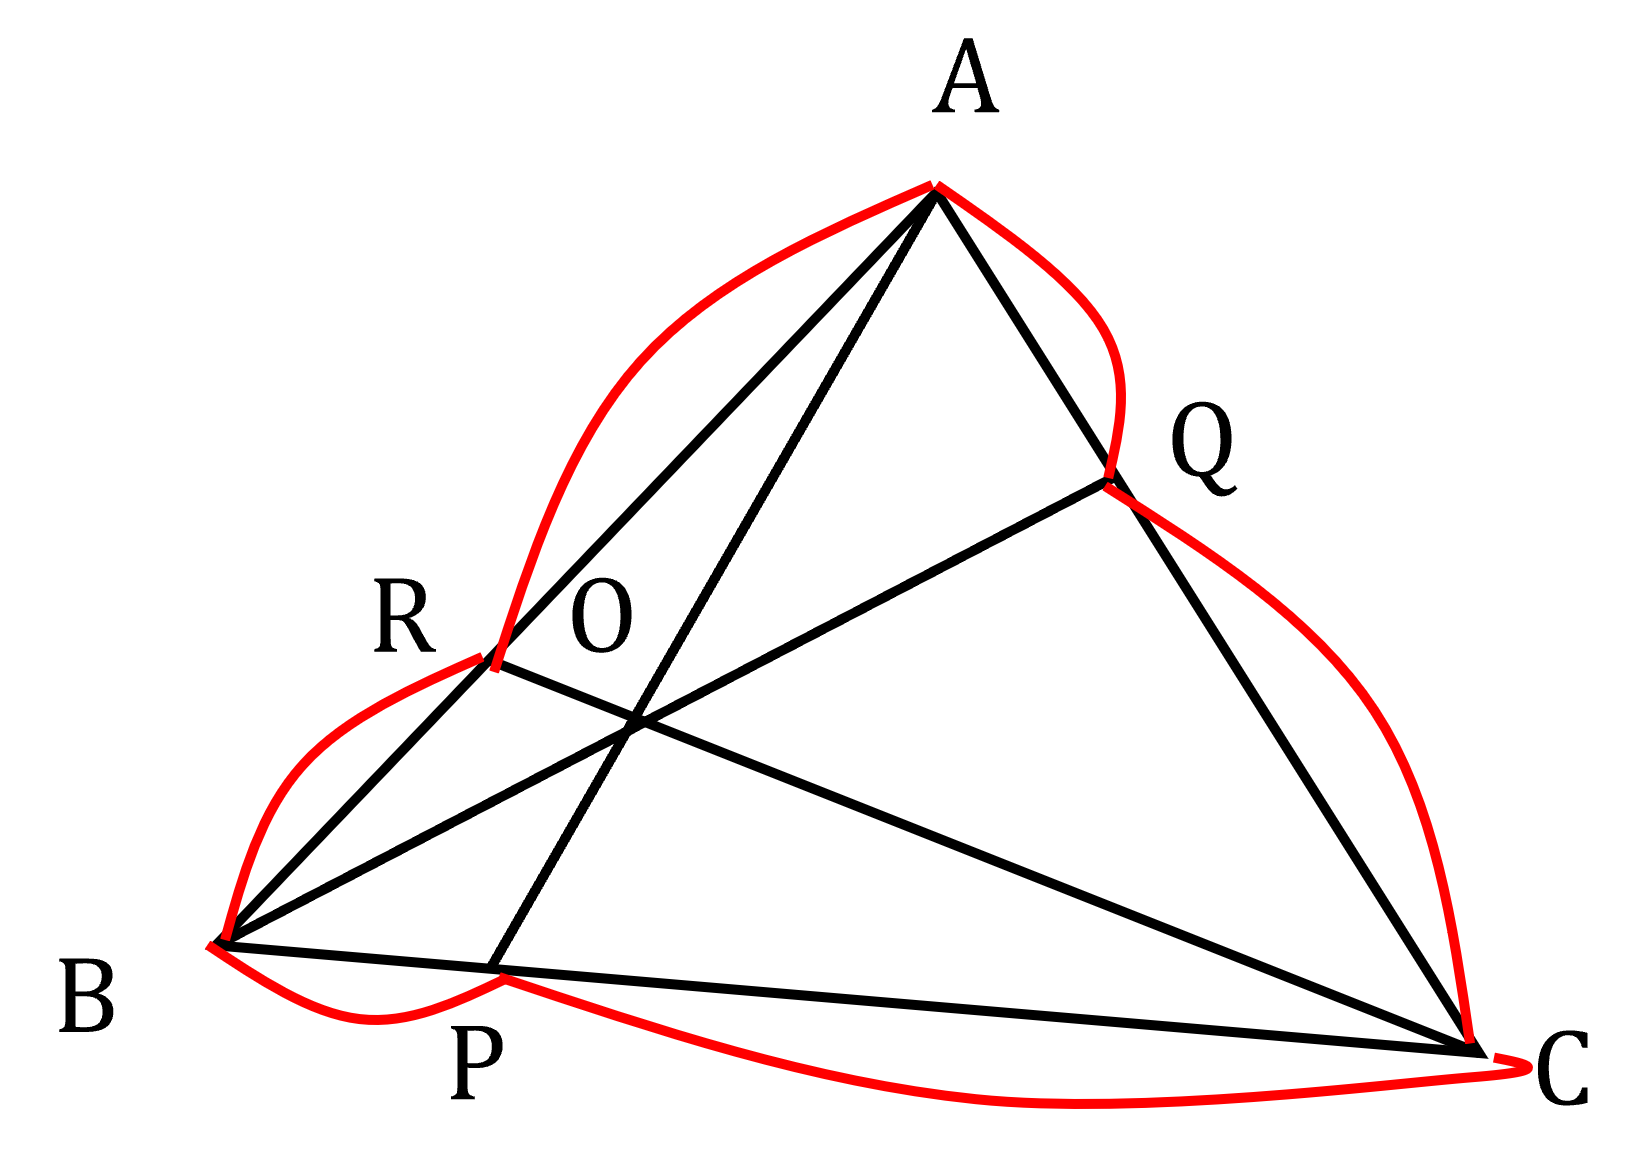
\includegraphics[width=100mm]{fig/3.png}
        \end{center}
    \end{figure}

\end{frame}
%---------------------------------------------------------------
\begin{frame}{三角比の定義}
    %! 三角比の定義, サインシータイコールr分のy, コサインシータイコールr分のx, タンジェントシータイコールx分のy
    \begin{eqnarray*}
        \sin \theta &=&\frac{y}{r} \\
        \cos \theta &=&\frac{x}{r} \\
        \tan \theta &=&\frac{y}{x}
    \end{eqnarray*}
    \begin{figure}[htbp]
        \begin{center}
            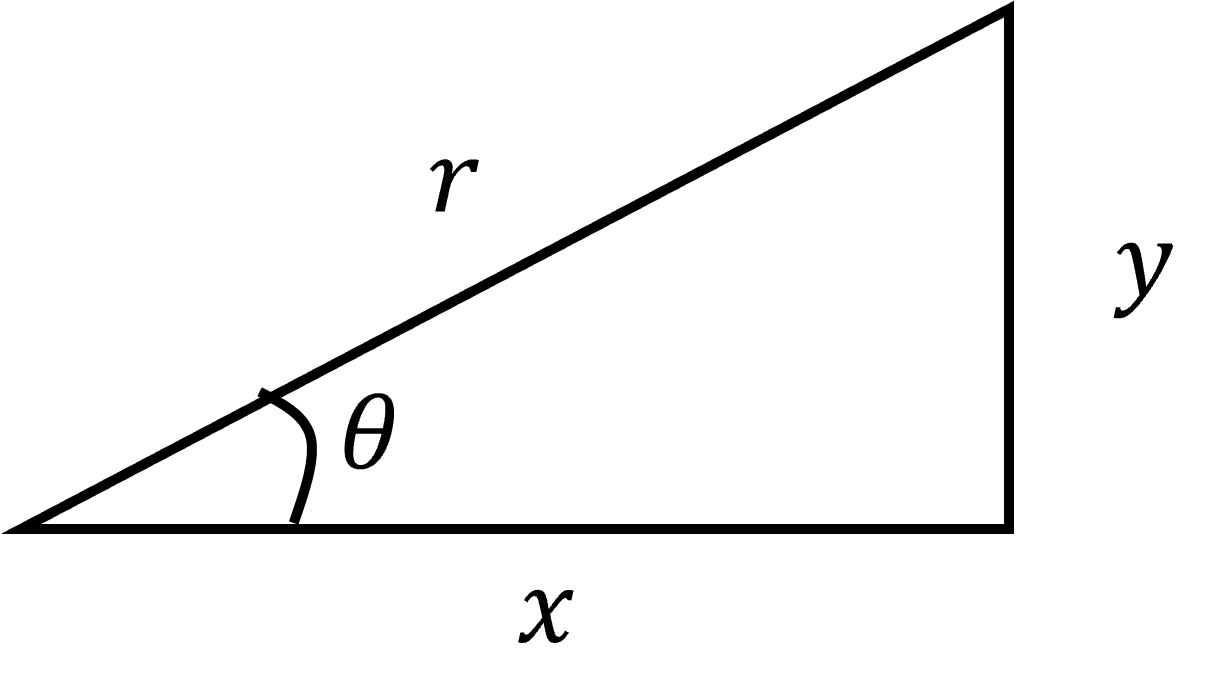
\includegraphics[width=40mm]{fig/4.png}
        \end{center}
    \end{figure}

\end{frame}
%---------------------------------------------------------------
\begin{frame}{三角比の相互関係}
    %! 三角比の相互関係, サイン2乗シータプラスコサイン2乗シータイコール1, タンジェントシータイコールコサインシータ分のサインシータ, 1プラスタンジェントシータ2乗イコールコサインシータ2乗分の1
    \begin{eqnarray*}
        \sin^2\theta + \cos^2\theta &=&1 \\
        \tan\theta &=& \frac{\sin\theta}{\cos\theta} \\
        1+\tan^2\theta&=&\frac{1}{\cos^2\theta}
    \end{eqnarray*}
\end{frame}
%---------------------------------------------------------------
\begin{frame}{$\pi-\theta$, $\frac{\pi}{2}\pm \theta$の三角比}
    %! パイマイナスシータ, 2分のパイプラスマイナスシータの三角比, サインパイプラスマイナスシータイコールプラスマイナスサインシータ, コサインパイプラスマイナスシータイコールマイナスプラスコサインシータ, タンジェントプラスマイナスシータイコールマイナスプラスコタンジェントシータ, サイン2分のパイプラスマイナスシータイコールコサインシータ, コサイン2分のパイプラスマイナスシータイコールマイナスプラスサインシータ, タンジェント2分のパイプラスマイナスシータイコールマイナスプラスタンジェントシータ分の1
    \begin{eqnarray*}
        \sin(\pi\pm\theta)&=&\pm\sin\theta \\
        \cos(\pi\pm\theta)&=&\mp\cos\theta \\
        \tan(\pi\pm\theta)&=&\mp\tan\theta \\
        \sin(\frac{\pi}{2}\pm\theta)&=&\cos\theta \\
        \cos(\frac{\pi}{2}\pm\theta)&=&\mp\sin\theta \\
        \tan(\frac{\pi}{2}\pm\theta)&=&\mp\frac{1}{\tan\theta} \\
    \end{eqnarray*}
\end{frame}
%---------------------------------------------------------------
\begin{frame}{正弦定理}
    %! 正弦定理, 三角形ABCの外接円の半径Rとするとサインa分のaイコール, サインb分のbイコールサインc分のcイコール2R
    $\bigtriangleup ABC$の外接円の半径を$R$とすると\par
    \begin{eqnarray*}
        \frac{a}{\sin A}=\frac{b}{\sin B}=\frac{c}{\sin C}=2R \\
    \end{eqnarray*}
    \begin{figure}[htbp]
        \begin{center}
            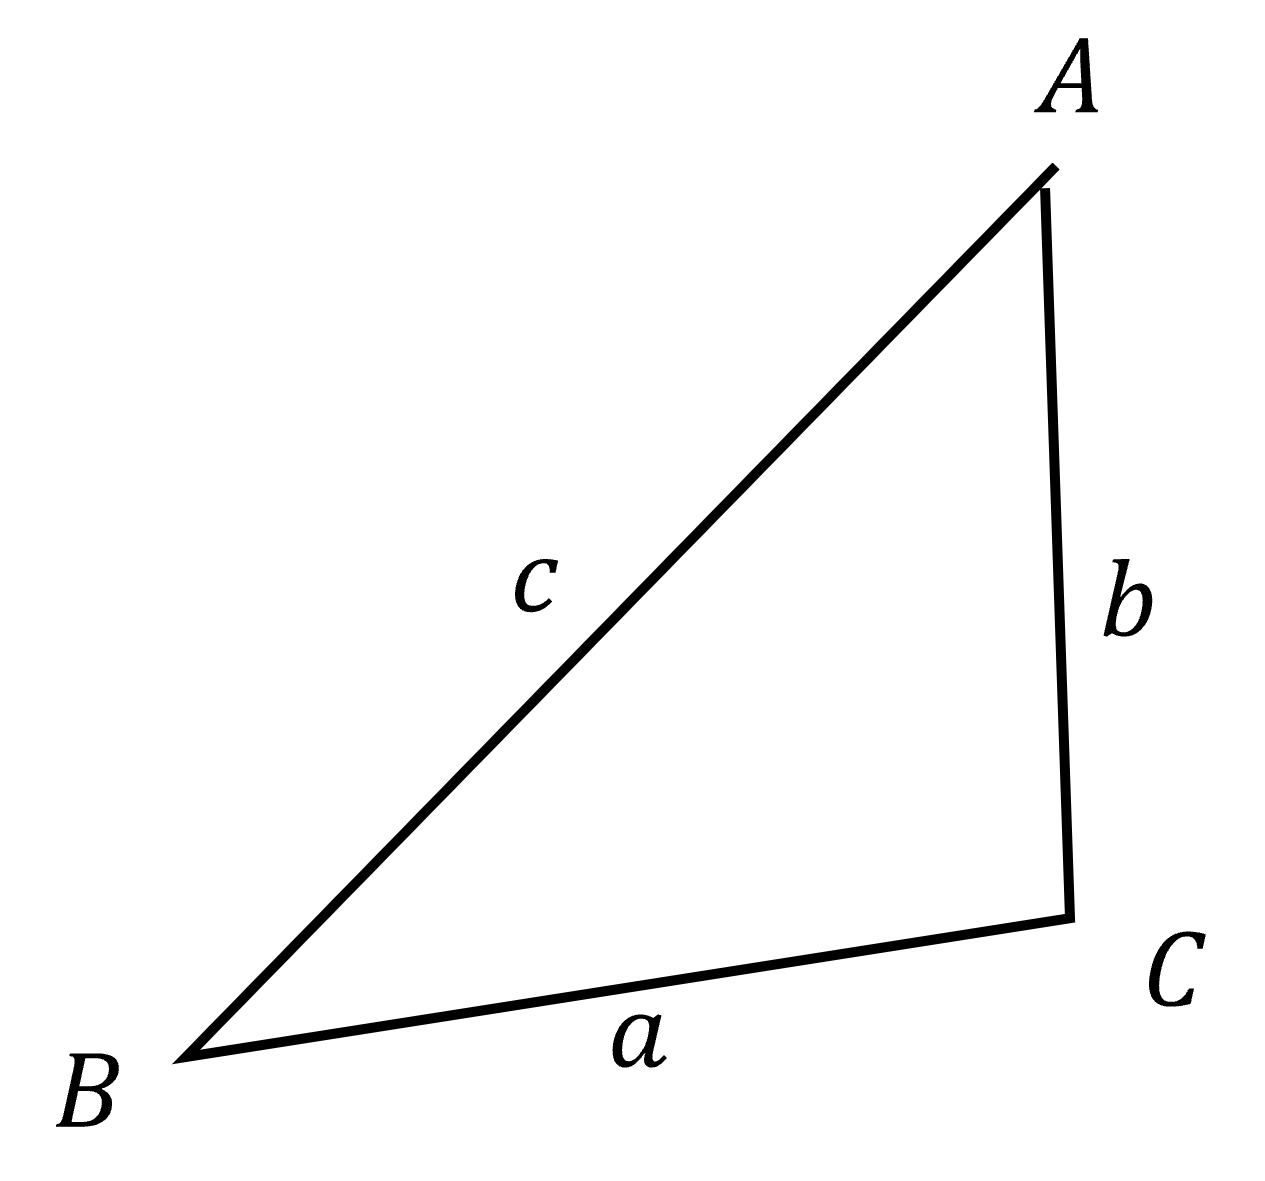
\includegraphics[width=40mm]{fig/5.png}
        \end{center}
    \end{figure}

\end{frame}
%---------------------------------------------------------------
\begin{frame}{余弦定理}
    %! 余弦定理, a2乗イコールb2乗プラスc2乗マイナス2bcコサインA, b2乗イコールc2乗プラスa2乗マイナス2caコサインB, c2乗イコールa2乗プラスb2乗マイナスabコサインC, aイコールcコサインBプラスbコサインC, bイコールaコサインCプラスcコサインA, cイコールbコサインAプラスaコサインB
    \begin{eqnarray*}
        a^2&=&b^2+c^2-2bc\cos A \\
        b^2&=&c^2+a^2-2ca\cos B \\
        c^2&=&a^2+b^2-2ab\cos C \\
        a&=&c\cos B+ b\cos C \\
        b&=&a\cos C+ c\cos A \\
        c&=&b\cos A+a\cos B
    \end{eqnarray*}
\end{frame}
%---------------------------------------------------------------
\begin{frame}{三角形の辺と角の関係}
    %! 三角形の辺と角の関係, 三角形の成立条件, 絶対値bマイナスcショウナリaショウナリbプラスc, 辺と角の大小関係, aショウナリb, 同値, AショウナリB, aイコールb, 同値, AイコールB, aダイナリb, 同値, AダイナリB, Aショウナリ2分のパイ, 同値, a2乗ショウナリb2乗プラスc2乗, Aイコール2分のパイ, 同値, a2乗イコールb2乗プラスc2乗, Aダイナリ2分のパイ, 同値, a2乗ダイナリb2乗プラスc2乗
    三角形の成立条件 $|b-c|<a<b+c$ \par
    辺と角の大小関係 \par
    \begin{eqnarray*}
        a<b &\Leftrightarrow& A<B \\
        a=b &\Leftrightarrow& A=B \\
        a>b &\Leftrightarrow& A>B \\
        A<\frac{\pi}{2} &\Leftrightarrow& a^2<b^2+c^2 \\
        A=\frac{\pi}{2} &\Leftrightarrow& a^2=b^2+c^2 \\
        A>\frac{\pi}{2} &\Leftrightarrow& a^2>b^2+c^2 \\
    \end{eqnarray*}
\end{frame}
%---------------------------------------------------------------
\begin{frame}{2辺とその間の角}
    %! 2辺とその間の角, 三角形ABCの面積SとするとSイコール2分の1bcサインA, イコール, 2分の1caサインB, イコール, 2分の1abサインC
    $\bigtriangleup ABC$の面積$S$とすると
    \begin{eqnarray*}
        S=\frac{1}{2}bc\sin A=\frac{1}{2}ca\sin B=\frac{1}{2}ab\sin C
    \end{eqnarray*}
\end{frame}
%---------------------------------------------------------------
\begin{frame}{3辺 (ヘロンの公式)}
    %! 3辺 (ヘロンの公式), Sイコール2分の1r括弧aプラスbプラスc
    \begin{eqnarray*}
        S=\frac{1}{2}r(a+b+c)
    \end{eqnarray*}
\end{frame}
%---------------------------------------------------------------
\begin{frame}{データの代表値}
    %! データの代表値, 平均xバーイコールn分の1シグマixi, 中央値メジアン, データの値の大きい順に並べたときの中央の位置にくる値, データの大きさが偶数のときは中央に並ぶ2つの値の平均値, 最頻値 (モード) , データにおける最も個数の多い値, 度数分布表に整理したときは度数が最も大きい階級の階級値
    平均値 :
    \begin{eqnarray*}
        \bar{x}=\frac{1}{n}\sum_i x_i
    \end{eqnarray*}
    中央値 (メジアン) : \par
    ・データを値の大きい順に並べたときの中央の位置にくる値\par
    ・データの大きさが偶数のときは中央に並ぶ2つの値の平均値\par
    最頻値 (モード) : \par
    ・データにおける最も個数の多い値 \par
    ・度数分布表に整理したときは度数が最も大きい階級の階級値
\end{frame}
%---------------------------------------------------------------
\begin{frame}{箱ひげ図}
    %! 箱ひげ図, データの最小値, 第1四分位数Q1, 中央値, 第3四分位数Q3, 最大値を箱と線(ひげ)で表現する図
    データの最小値, 第1四分位数$Q_1$, 中央値, 第3四分位数$Q_3$, 最大値を\par
    箱と線(ひげ)で表現する図 \par
    \begin{figure}[htbp]
        \begin{center}
            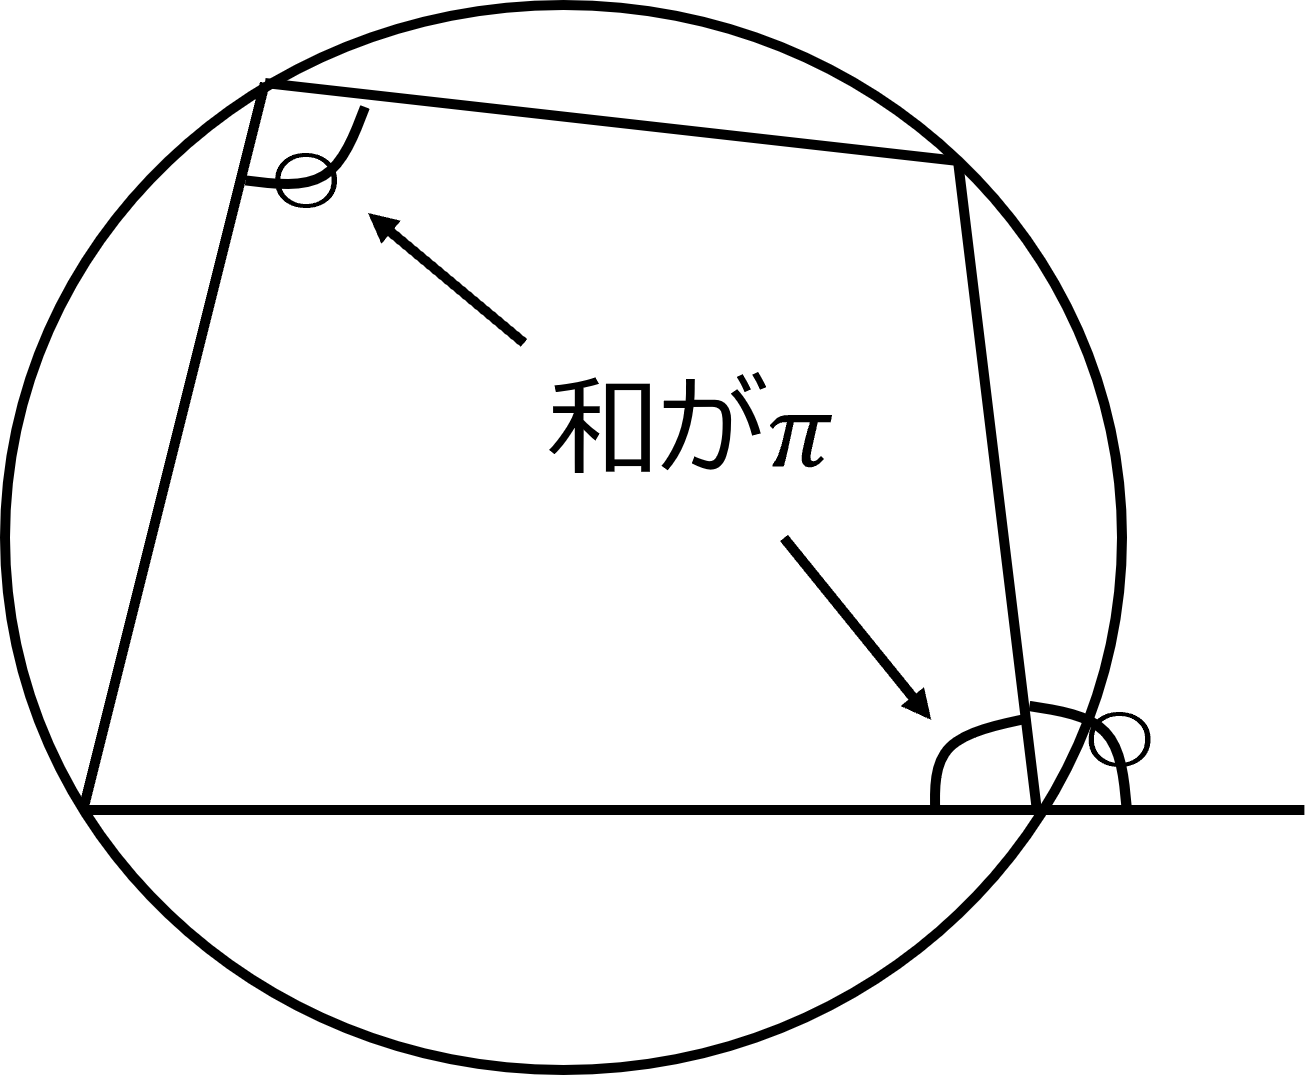
\includegraphics[width=40mm]{fig/6.png}
        \end{center}
    \end{figure}
\end{frame}
%---------------------------------------------------------------
\begin{frame}{偏差: 変数$x_i$と平均$\bar{x}$の差}
    %! 偏差: 変数と平均の差, xiマイナスxバー
    \begin{eqnarray*}
        x_i-\bar{x}
    \end{eqnarray*}
\end{frame}
%---------------------------------------------------------------
\begin{frame}{分散: 偏差2乗平均}
    %! 分散: 偏差2乗平均, シグマ2乗イコールn分の1シグマi括弧xiマイナスxバー2乗イコールx2乗バーマイナスxバー2乗
    \begin{eqnarray*}
        \sigma^2=\frac{1}{n}\sum_i (x_i-\bar{x})^2=\bar{x^2}-\bar{x}^2
    \end{eqnarray*}
\end{frame}
%---------------------------------------------------------------
\begin{frame}{標準偏差: 分散の正の平方根}
    %! 標準偏差: 分散の正の平方根, シグマイコールルートn分の1シグマi括弧xiマイナスxバー2乗
    \begin{eqnarray*}
        \sigma=\sqrt{\frac{1}{n}\sum_i (x_i-\bar{x})^2}
    \end{eqnarray*}
\end{frame}
%---------------------------------------------------------------
\begin{frame}{相関係数}
    %! 相関係数, 変量x, yの標準偏差をそれぞれシグマx, シグマyとし, xとyの共分散をシグマxyとすると, 相関係数rイコールシグマxシグマy分のシグマxy, ただし, マイナス1ショウナリrショウナリ1, ここでシグマxyイコールn分の1シグマi括弧xiマイナスxバー括弧yiマイナスyバー, rイコール, ルートn分の1シグマi括弧xiマイナスxバー2乗, ルートn分の1シグマi括弧yiマイナスyバー2乗, 分のn分の1シグマi括弧xiマイナスxバー括弧yiマイナスyバー, イコール, ルートシグマi括弧xiマイナスxバー2乗, ルートシグマi括弧yiマイナスyバー2乗, 分のシグマi括弧xiマイナスxバー括弧yiマイナスyバー
    変量$x$, $y$の標準偏差をそれぞれ$\sigma_x$, $\sigma_y$とし, \par
    $x$と$y$の共分散を$\sigma_{xy}$とすると \par
    \begin{eqnarray*}
        r&=&\frac{\sigma_{xy}}{\sigma_x\sigma_y} (-1\leq r \leq 1) \\
        \sigma_{xy}&=&\frac{1}{n}\sum_i(x_i-\bar{x})(y_i-\bar{y}) \\
        r&=&\frac{\frac{1}{n}\sum_i(x_i-\bar{x})(y_i-\bar{y})}{\sqrt{\frac{1}{n}\sum_i(x_i-\bar{x})^2}\sqrt{\frac{1}{n}\sum_i(y_i-\bar{y})^2}} \\
        &=&\frac{\sum_i(x_i-\bar{x})(y_i-\bar{y})}{\sqrt{\sum_i(x_i-\bar{x})^2\sum_i(y_i-\bar{y})^2}}
    \end{eqnarray*}
\end{frame}

\end{document}
